\documentclass[12pt]{extarticle}
\usepackage{tempora}
\usepackage[T1, T2A]{fontenc}
\usepackage[utf8]{inputenc}
\usepackage[english, ukrainian]{babel}
\usepackage{geometry}
\usepackage{graphicx}
\usepackage{multirow}
\usepackage{multicol}
\usepackage{float}
\graphicspath{{/home/artem/Pictures}}
\geometry
{
    a4paper,
    left=30mm,
    top=15mm,
    right=20mm,
    bottom=15mm,
}

\begin{document}
\begin{titlepage}
    \begin{center}
        \textbf{\normalsize{\MakeUppercase{
            Міністерство Освіти і науки України
            Національний університет "Львівська політехніка"
        }}}

        \begin{flushright}
        \textbf{ІКНІ}\\
        Кафедра \textbf{ПЗ}
        \end{flushright}
        \vspace{15mm}

        \includegraphics[width=0.4\textwidth]{lpnu_logo.png}

        \vspace*{\fill}

        \textbf{\normalsize{\MakeUppercase{Звіт}}}
            
        До лабораторної роботи №6

        \textbf{на тему:} “Багатопоточність в операційній системі Linux. Створення,
        керування та синхронізація потоків”

        \textbf{з дисципліни:} “Операційні системи”
            
        \vspace*{\fill}

        \begin{flushright}

            \textbf{Лектор:}\\
            старший викладач кафедри ПЗ\\
            Грицай О.Д.\\
            \vspace{12pt}

            \textbf{Виконав:}\\
            студент групи ПЗ-24\\
            Губик А. С.\\
            \vspace{12pt}

            \textbf{Прийняв:}\\
            доцент кафедри ПЗ\\
            Горечко О. М.\\
        \vspace{12pt}
        \end{flushright}

        Львів -- 2023
            
            
    \end{center}
\end{titlepage}

\textbf{Тема роботи:}Багатопоточність в операційній системі Linux. Створення,
керування та синхронізація потоків
\vspace{12pt}

\textbf{Мета роботи:}Навчитися створювати потоки та керувати ними в операційній
системі Linux. Ознайомитися з методами синхронізації потоків в операційній
системі Linux. Навчитися реалізовувати багатопоточний алгоритм розв’язку
задачі з використанням синхронізації в операційній системі Linux.

\subsection*{Теоретичні відомості}
Потоки в операційній системі Linux. Поняття потоку, як одиниці
виконання процесу в операційній системі (ОС) Linux, аналогічне як і у ОС
Windows. Кожен процес можна представити як контейнер ресурсів і
послідовність інструкцій виконання. Таким чином, можна сказати, що кожен
процес містить хоча б один потік виконання, якому надані лічильник
інструкцій, регістри і стек. Крім того, у кожному процесі можна створити
додаткові гілки виконання – потоки, тоді такий процес називають
багатопоточним.
Різниця між потоками в ОС Linux і в ОС Windows полягає у їх
представленні в ядрі операційних систем. В ОС Windows потоки виконання у
режимі користувача зіставляються з потоками у режим ядра. У перших версіях
ядра Linux потоки користувача зіставлялись з процесами у ядрі. Створення
потоку відбувалось з допомогою системного виклику clone(). Виклик clone(), як
і fork() дозволяє створювати новий процес, але з певними відмінностями :
- одразу повне копіювання батьківського процесу
- створення власного стеку
- необхідно вказати спеціальний набір прапорців успадкування для того,
щоб визначити, як будуть розподілятися ресурси (адресний простір, відкритті
файли, обробники сигналів) між батьківським і дочірнім процесом.
Таким чином, створювався новий потік у режимі користувача, який
відобрається у процес ядра. Відображення здійснюється за моделлю 1:1.
Оскільки керуючий блок процесу в Linux представлений в ядрі структурою
Фактично у ядрі потоки і процеси не розрізнялися. Але системний виклик
clone() не підтримувався стандартом POSIX і тому розроблялись бібліотеки
потоків, що дозволяли працювати з потоками, використовуючи clone() з
різними атрибутами виконання.
У сучасних версіях Linux підтримуються спеціальні об'єкти ядра - потоки
ядра, побудованні на зміненному і розширеному системному виклику clone().
Підтримка потоків здійснюється через POSIX-сумісну бібліотеку NPTL (Native
POSIX Threads Library). Типи даних і функції, що застосовуються до потоків

\subsection*{Індивідуальне завдання}

3. Бінарний пошук заданого елементу масиву (кількість елементів >10000,
елементи рандомні). Вивести значення та індекс. (Синхронізація: м’ютекс,
умовні змінні)

\paragraph{I.} Розпаралелення бінарного пошуку на 2, 4, 8, 16 потоків


\begin{figure}[H]
    \centering
    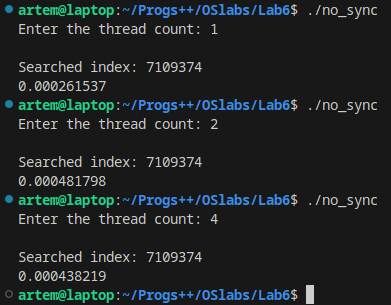
\includegraphics[width=0.90\textwidth]{console}
    \caption{Графік залежності швидкості роботи програми від кількості потоків}
\end{figure}
\begin{figure}[H]
    \centering
    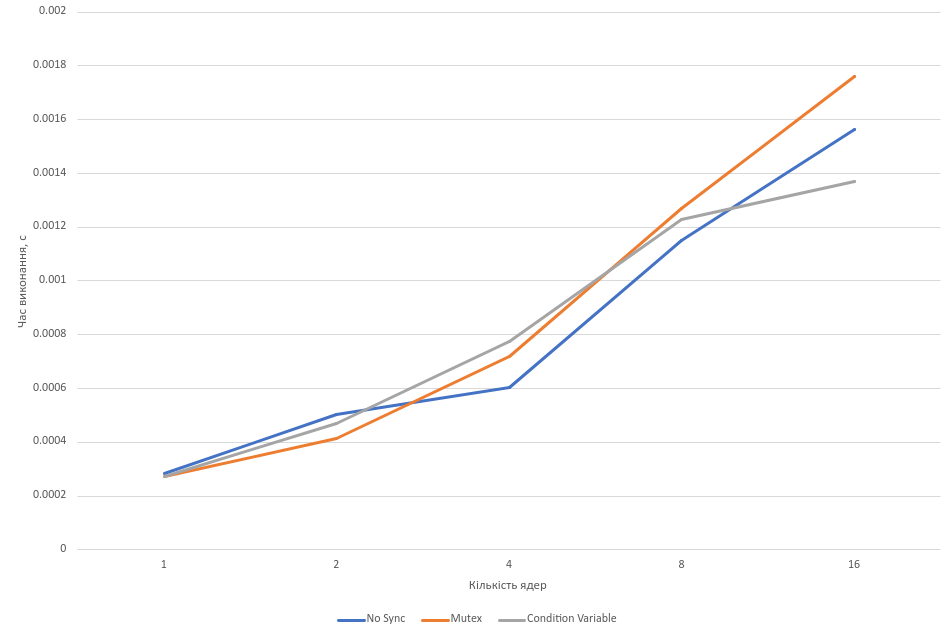
\includegraphics[width=0.90\textwidth]{graph}
    \caption{Графік залежності швидкості роботи програми від кількості потоків}
\end{figure}

Як бачимо синхронізація сповільнює роботу і не впливає на правильність виконання бінарного пошуку.



\paragraph{II.} Задання пріоритету, відміна та affinity
\begin{figure}[H]
    \centering
    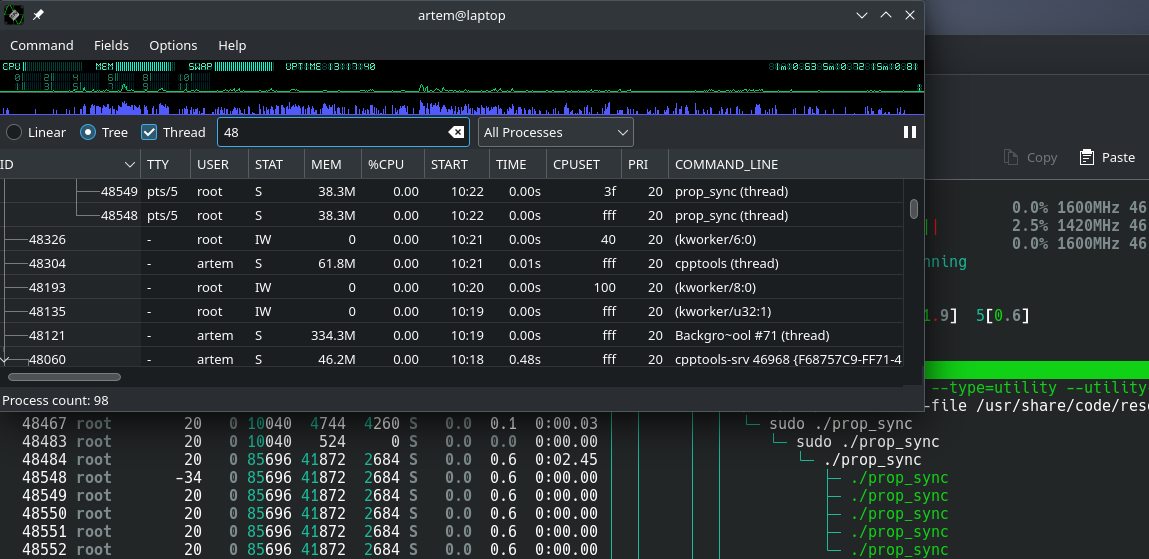
\includegraphics[width=0.90\textwidth]{aff}
    \caption{}
\end{figure}

\textbf{Висновок:}
Я ознайомився з бібліотекою POSIX Threads.
Ефективність синхронізації залежить від поставленої перед нами задачі. У
випадку з бінарним пошуком воно не потрібне і сповільнює роботу.
 \end{document}
